\chapter{Cloture Phase}
\newpage
\begin{center}
    \centering
    \LARGE\textbf{Introduction} 
     \vspace{1cm} \\
   \raggedright
\end{center}
\addcontentsline{toc}{section}{Introduction}
In this final chapter, we will explain the ultimate phase of a development cycle using Scrum.  
First, we will start by listing the hardware and software development environment that we used during the realization of our project.  
Then, we will present a deployment diagram that shows the architecture of our application, as well as a schematic representation of the various tasks carried out throughout the project.
\section{Development Environment}
To begin, we will present the hardware and software environment that we are using.
\subsection{Hardware Environment}
Here are the specifications of the machines we used:
\begin{table}[h]
\centering
\begin{tabular}{|l|>{\centering\arraybackslash}p{5cm}|>{\centering\arraybackslash}p{5cm}|}
\hline
\textbf{Computer} & \textbf{1} & \textbf{2} \\ \hline
Owner & Nourchene GARBOUJ & Yassine BEN YEDDER \\ \hline
Processor & Core i3 & Core i5 \\ \hline
RAM & 8 Go & 8 Go \\ \hline
SSD & 256 GB & 256 GB \\ \hline
Operating System & Windows 10 Professional 64-bit & Windows 10 Professional 64-bit \\ \hline
\end{tabular}
\caption{Hardware Environment}
\end{table}
\subsection{Software Environment}

\begin{figure}[h]
\centering
\begin{minipage}{0.3\textwidth}
    \centering
    
\includegraphics[width=\linewidth,frame]{figures/drawio.png}
    \caption{Draw.io}
\end{minipage}
\hfill
\begin{minipage}{0.6\textwidth}
    \textbf{Draw.io} is a technology stack for building diagramming applications, and the world’s most widely used browser-based end-user diagramming software.\\Their mission statement is \textit{“provide free, high quality diagramming software for everyone”}\cite{samplewebs9}
\end{minipage}
\end{figure}

\begin{figure}[h]
\centering
\begin{minipage}{0.3\textwidth}
    \centering
    
\includegraphics[width=\linewidth,frame]{figures/overleaf.png}
    \caption{Overleaf}
\end{minipage}
\hfill
\begin{minipage}{0.6\textwidth}
   \textbf{LaTeX} is a typesetting system and Overleaf is a company that provides a web server that hosts Linux docker containers on which you can run LaTeX.\cite{samplewebs10}
\end{minipage}
\end{figure}

\begin{figure}[h]
\centering
\begin{minipage}{0.3\textwidth}
    \centering
    
\includegraphics[width=\linewidth,frame]{figures/balsamiq.png}
    \caption{Balsamiq Wireframes}
\end{minipage}
\hfill
\begin{minipage}{0.6\textwidth}
   \textbf{Balsamiq Wireframes} is a user interface design tool for creating wireframes (sometimes called mock-ups or low-fidelity prototypes). You can use it to generate digital sketches of your idea or concept for an application or website, to facilitate discussion and understanding before any code is written.\cite{samplewebs11}
\end{minipage}
\end{figure}

\begin{figure}[h]
\centering
\begin{minipage}{0.3\textwidth}
    \centering
    
\includegraphics[width=\linewidth,frame]{figures/postman.png}
    \caption{Postman}
\end{minipage}
\hfill
\begin{minipage}{0.6\textwidth}
  \textbf{Postman} is the single platform for designing, building, and scaling APIs—together. Join over 35 million developers who have consolidated their workflows and leveled up their API game—all in one powerful platform.\cite{samplewebs12}
\end{minipage}
\end{figure}

\begin{figure}[h]
\centering
\begin{minipage}{0.3\textwidth}
    \centering
    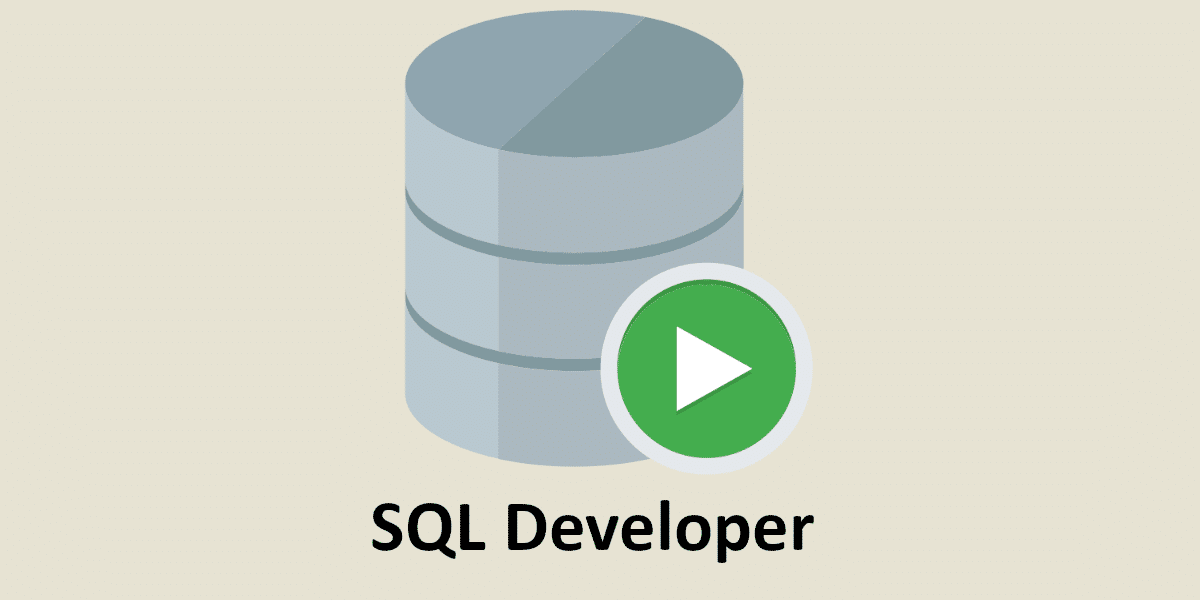
\includegraphics[width=\linewidth,frame]{figures/sql developer.png}
    \caption{Oracle SQL Developer}
\end{minipage}
\hfill
\begin{minipage}{0.6\textwidth}
  \textbf{Oracle SQL Developer} is a free, development environment that simplifies the management of Oracle Database in both traditional and Cloud deployments.\cite{samplewebs13}
\end{minipage}
\end{figure}

\begin{figure}[h]
\centering
\begin{minipage}{0.3\textwidth}
    \centering
    
\includegraphics[width=\linewidth,frame]{figures/oracle database.png}
    \caption{Oracle Database}
\end{minipage}
\hfill
\begin{minipage}{0.6\textwidth}
  An \textbf{Oracle database} is a fully configurable and scalable enterprise database solution that uses a relational model for information management.\cite{samplewebs14}
\end{minipage}
\end{figure}

\begin{figure}[h]
\centering
\begin{minipage}{0.3\textwidth}
    \centering
    
\includegraphics[width=\linewidth,frame]{figures/vs code.png}
    \caption{VS Code}
\end{minipage}
\hfill
\begin{minipage}{0.6\textwidth}
  The \textbf{Visual Studio} IDE is a creative launching pad that you can use to edit, debug, and build code, and then publish an app. Over and above the standard editor and debugger that most IDEs provide, Visual Studio includes compilers, code completion tools, graphical designers, and many more features to enhance the software development process.\cite{samplewebs15}
\end{minipage}
\end{figure}

\begin{figure}[h]
\centering
\begin{minipage}{0.3\textwidth}
    \centering
    
\includegraphics[width=\linewidth,frame]{figures/node.png}
    \caption{Node.js}
\end{minipage}
\hfill
\begin{minipage}{0.6\textwidth}
  \textbf{Node.js®} is a free, open-source, cross-platform JavaScript runtime environment that lets developers create servers, web apps, command line tools and scripts.\cite{samplewebs18}
\end{minipage}
\end{figure}

\begin{figure}[h]
\centering
\begin{minipage}{0.3\textwidth}
    \centering
    
\includegraphics[width=\linewidth,frame]{figures/react.png}
    \caption{REACT.js}
\end{minipage}
\hfill
\begin{minipage}{0.6\textwidth}
  React is the library for web and native user interfaces. Build user interfaces out of individual pieces called components written in JavaScript.\cite{samplewebs16}
\end{minipage}
\end{figure}

\begin{figure}[h]
\centering
\begin{minipage}{0.3\textwidth}
    \centering
    
\includegraphics[width=\linewidth,frame]{figures/express.png}
    \caption{Express.js}
\end{minipage}
\hfill
\begin{minipage}{0.6\textwidth}
  \textbf{Express} is a minimal and flexible Node.js web application framework that provides a robust set of features for web and mobile applications.\cite{samplewebs17}
\end{minipage}
\end{figure}

\begin{figure}[h]
\centering
\begin{minipage}{0.3\textwidth}
    \centering
    
\includegraphics[width=\linewidth,frame]{figures/tailwind.png}
    \caption{Node.js}
\end{minipage}
\hfill
\begin{minipage}{0.6\textwidth}
  \textbf{Tailwind CSS} is A utility-first CSS framework packed with classes like flex, pt-4, text-center and rotate-90 that can be composed to build any design, directly in your markup.\cite{samplewebs19}
\end{minipage}
\end{figure}

\begin{figure}[h]
\centering
\begin{minipage}{0.3\textwidth}
    \centering
    
\includegraphics[width=\linewidth,frame]{figures/paperless.png}
    \caption{Paperless NGX}
\end{minipage}
\hfill
\begin{minipage}{0.6\textwidth}
 \textbf{Paperless-ngx} is a community-supported open-source document management system that transforms your physical documents into a searchable online archive so you can keep, well, less paper.\cite{samplewebs20}
\end{minipage}
\end{figure}

\begin{figure}[h]
\centering
\begin{minipage}{0.3\textwidth}
    \centering
    
\includegraphics[width=\linewidth,frame]{figures/redis.png}
    \caption{Redis}
\end{minipage}
\hfill
\begin{minipage}{0.6\textwidth}
Most people think \textbf{Redis} is just for caching... Redis is a versatile Vector Database, primarily known for its speed, and flexibility.\cite{samplewebs21}
\end{minipage}
\end{figure}

\begin{figure}[h]
\centering
\begin{minipage}{0.3\textwidth}
    \centering
    
\includegraphics[width=\linewidth,frame]{figures/jwt.png}
    \caption{JWT}
\end{minipage}
\hfill
\begin{minipage}{0.6\textwidth}
\textbf{JSON Web Token (JWT)} is an open standard (RFC 7519) that defines a compact and self-contained way for securely transmitting information between parties as a JSON object. This information can be verified and trusted because it is digitally signed. JWTs can be signed using a secret (with the HMAC algorithm) or a public/private key pair using RSA or ECDSA.\cite{samplewebs22}
\end{minipage}
\end{figure}

\begin{figure}[h]
\centering
\begin{minipage}{0.3\textwidth}
    \centering
    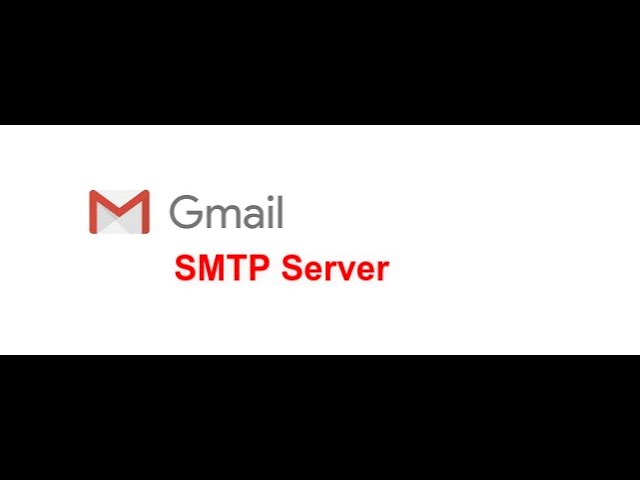
\includegraphics[width=\linewidth,frame]{figures/smtp.jpg}
    \caption{Google SMTP}
\end{minipage}
\hfill
\begin{minipage}{0.6\textwidth}
In simple terms, \textbf{SMTP (Simple Mail Transfer Protocol)} is an email protocol used by mail servers for outgoing emails over the Internet. Email protocols, on the other hand, are specific rules that organize the email exchange between email clients and accounts. This particular protocol serves to handle email sending through an SMTP server.\cite{samplewebs23}
\end{minipage}
\end{figure}

\begin{figure}[h]
\centering
\begin{minipage}{0.3\textwidth}
    \centering
    
\includegraphics[width=\linewidth,frame]{figures/openaiapi.png}
    \caption{Open AI API}
\end{minipage}
\hfill
\begin{minipage}{0.6\textwidth}
\textbf{OpenAI API} (Application Programming Interface) serves as a bridge to OpenAI's powerful machine learning models, allowing you to integrate cutting-edge AI capabilities into your projects with relative ease.\cite{samplewebs24}
\end{minipage}
\end{figure}

\begin{figure}[h]
\centering
\begin{minipage}{0.3\textwidth}
    \centering
    
\includegraphics[width=\linewidth,frame]{figures/chartjs.jpg}
    \caption{Chart.js}
\end{minipage}
\hfill
\begin{minipage}{0.6\textwidth}
\textbf{Chart.js} Simple yet flexible JavaScript charting library for the modern web\cite{samplewebs25}
\end{minipage}
\end{figure}

\begin{figure}[h]
\centering
\begin{minipage}{0.3\textwidth}
    \centering
    
\includegraphics[width=\linewidth,frame]{figures/uuid.png}
    \caption{UUID}
\end{minipage}
\hfill
\begin{minipage}{0.6\textwidth}
\textbf{A Universally Unique Identifier (UUID)} is a label used to uniquely identify a resource among all other resources of that type.\cite{samplewebs26}
\end{minipage}
\end{figure}

\begin{figure}[h]
\centering
\begin{minipage}{0.3\textwidth}
    \centering
    
\includegraphics[width=\linewidth,frame]{figures/docker.png}
    \caption{Docker}
\end{minipage}
\hfill
\begin{minipage}{0.6\textwidth}
\textbf{Docker} is a software platform that allows you to build, test, and deploy applications quickly. Docker packages software into standardized units called containers that have everything the software needs to run including libraries, system tools, code, and runtime.\cite{samplewebs27}
\end{minipage}
\end{figure}

\begin{figure}[h]
\centering
\begin{minipage}{0.3\textwidth}
    \centering
    
\includegraphics[width=\linewidth,frame]{figures/jira logo.png}
    \caption{Jira}
\end{minipage}
\hfill
\begin{minipage}{0.6\textwidth}
\textbf{Jira} is the number 1 agile project management tool used by teams to plan, track, release and support world-class software with confidence. It is the single source of truth for your entire development life-cycle, empowering autonomous teams with the context to move quickly while staying connected to the greater business goal.\cite{samplewebs28}
\end{minipage}
\end{figure}

\begin{figure}[h]
\centering
\begin{minipage}{0.3\textwidth}
    \centering
    
\includegraphics[width=\linewidth,frame]{figures/github.png}
    \caption{Github}
\end{minipage}
\hfill
\begin{minipage}{0.6\textwidth}
\textbf{GitHub} is a cloud-based platform where you can store, share, and work together with others to write code. Storing your code in a "repository" on GitHub allows you to: Showcase or share your work. Track and manage changes to your code over time.\cite{samplewebs29}
\end{minipage}
\end{figure}
\clearpage
\section{Technological Choices}
\subsection{The MVC Architecture}
One of the most famous design patterns is called MVC, which stands for Model - View - Controller.
The MVC pattern helps organize your source code effectively. It guides you in knowing which files to create, but more importantly, it defines the role of each. The goal of MVC is precisely to separate the logic of the code into three parts, each found in separate files.

\begin{itemize}
    \item Model: This part manages the data of your website. Its role is to retrieve the "raw" information from the database, organize it, and assemble it so that it can then be processed by the controller. Typically, it includes SQL queries, among other things.
    \item View: This part focuses on display. It performs almost no calculations and simply uses variables to determine what to show. It mainly contains HTML code, but also some very simple PHP loops and conditions, for example, to display a list of messages.
    \item Controller: This part manages the logic that makes decisions. It acts as the intermediary between the model and the view: the controller requests data from the model, analyzes it, makes decisions, and sends the content to be displayed to the view. The controller contains PHP code exclusively. It also determines, for example, whether the visitor has the right to access the page (access control).
\end{itemize}
 \begin{figure}[h]
    \centering
    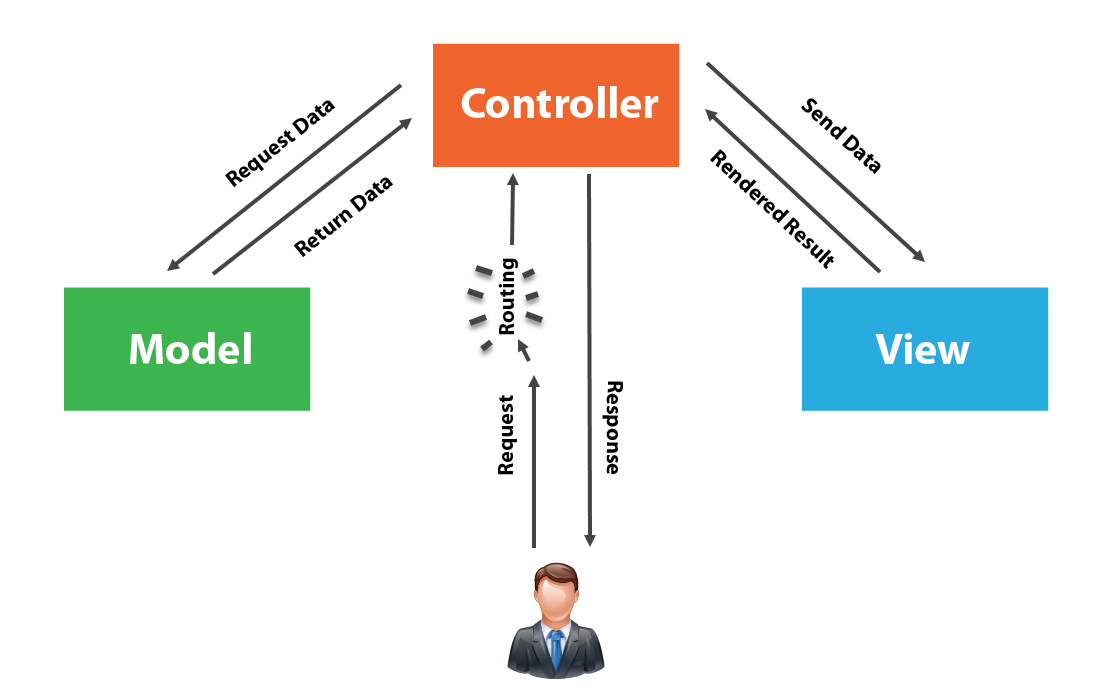
\includegraphics[width=0.9\textwidth]{figures/mvc.png} 
    \caption{The MVC Architecture.}
\end{figure}\
\clearpage
\subsection{Deployment Diagram}
A deployment diagram allows you to illustrate how instances of software systems and/or containers in the static model are deployed on to the infrastructure within a given deployment environment (e.g. production, staging, development, etc). It’s based upon a UML deployment diagram.\cite{samplewebs30}
\begin{figure}[h]
    \centering
    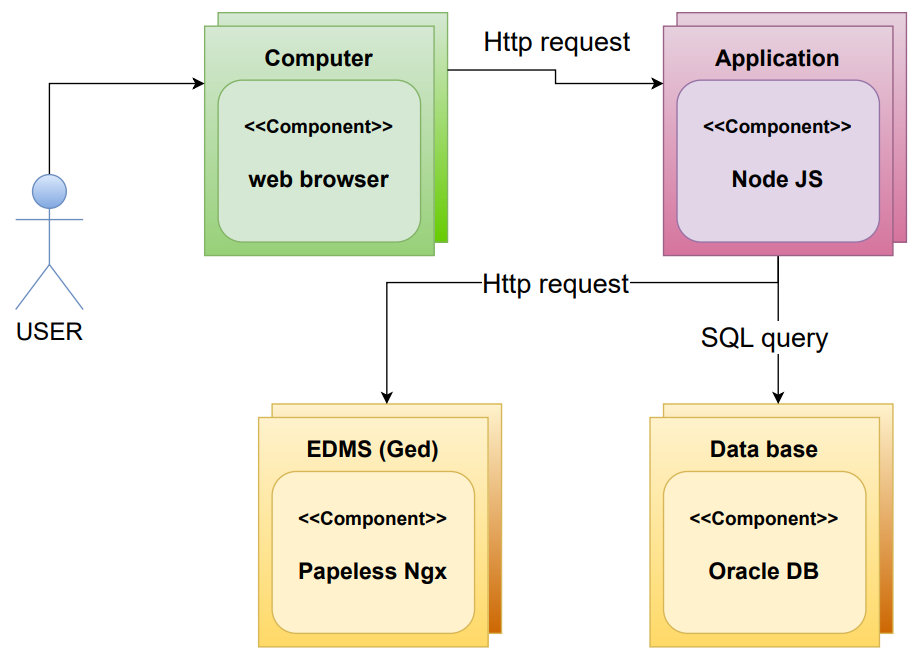
\includegraphics[width=0.9\textwidth]{figures/diagram de deploiement.png} 
    \caption{Deployment Diagram.}
\end{figure}\
\section{Project Management}
\subsection{Task Table}
We will present a few screenshots demonstrating the distribution of tasks at specific moments during the implementation of our project.
\begin{figure}[h]
    \centering
    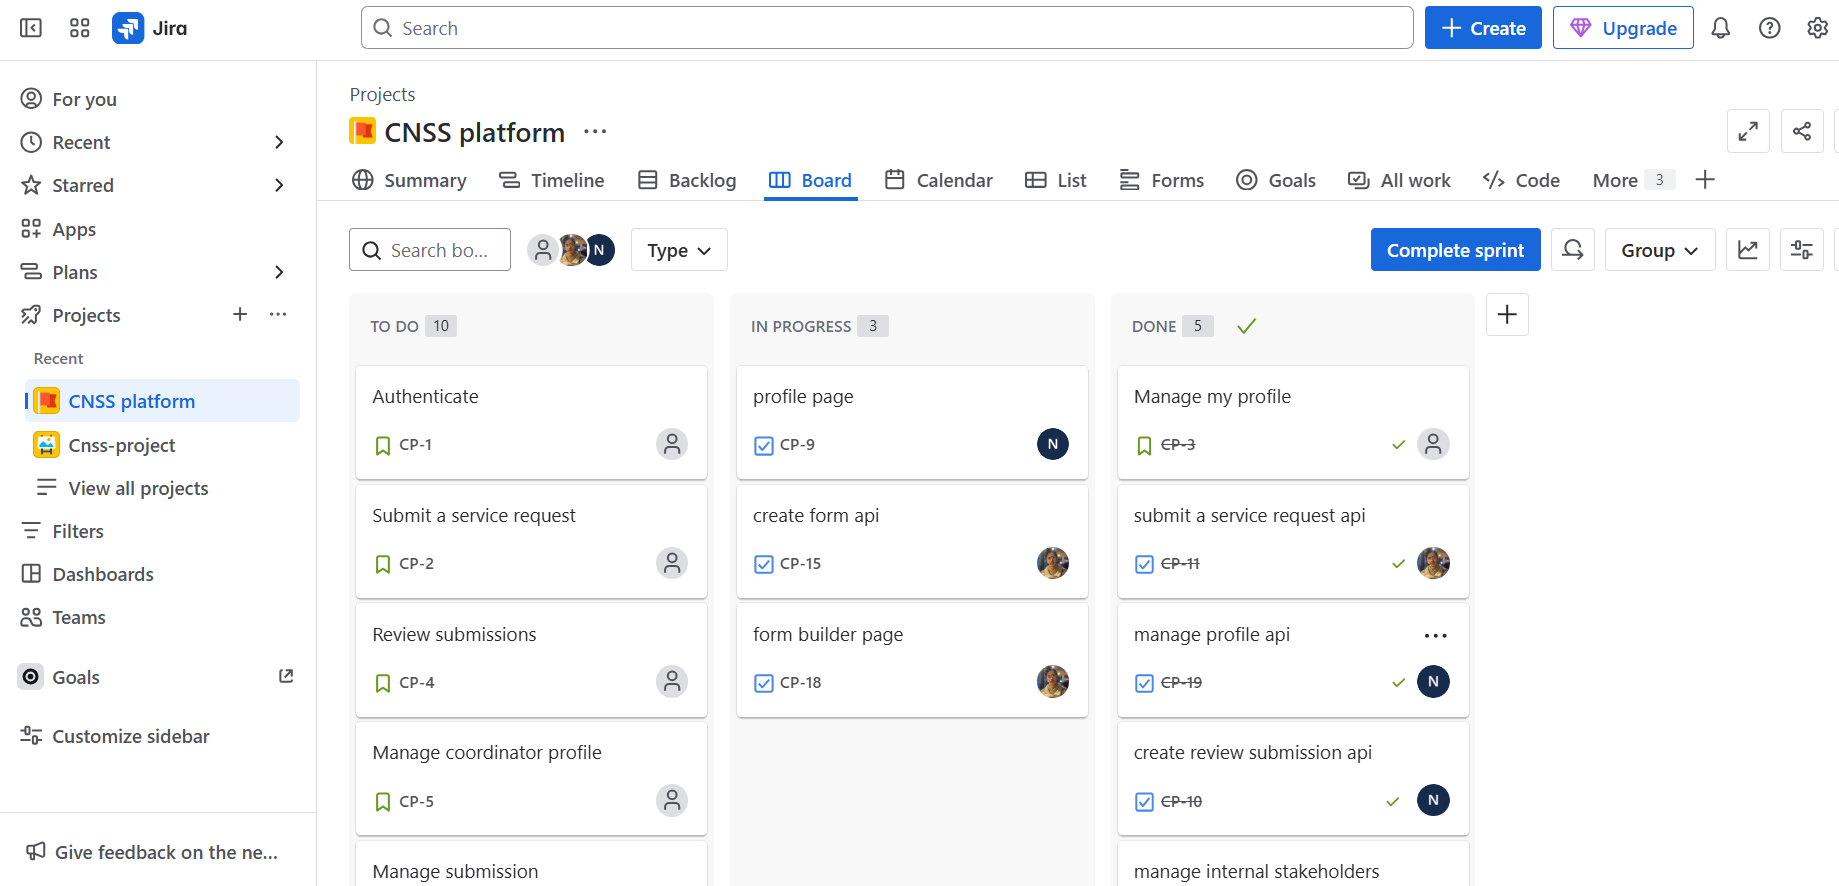
\includegraphics[width=0.9\textwidth]{figures/sprint1 jira.png} 
    \caption{Task distribution for the first sprint using Jira.}
\end{figure}\
\begin{figure}[h]
    \centering
    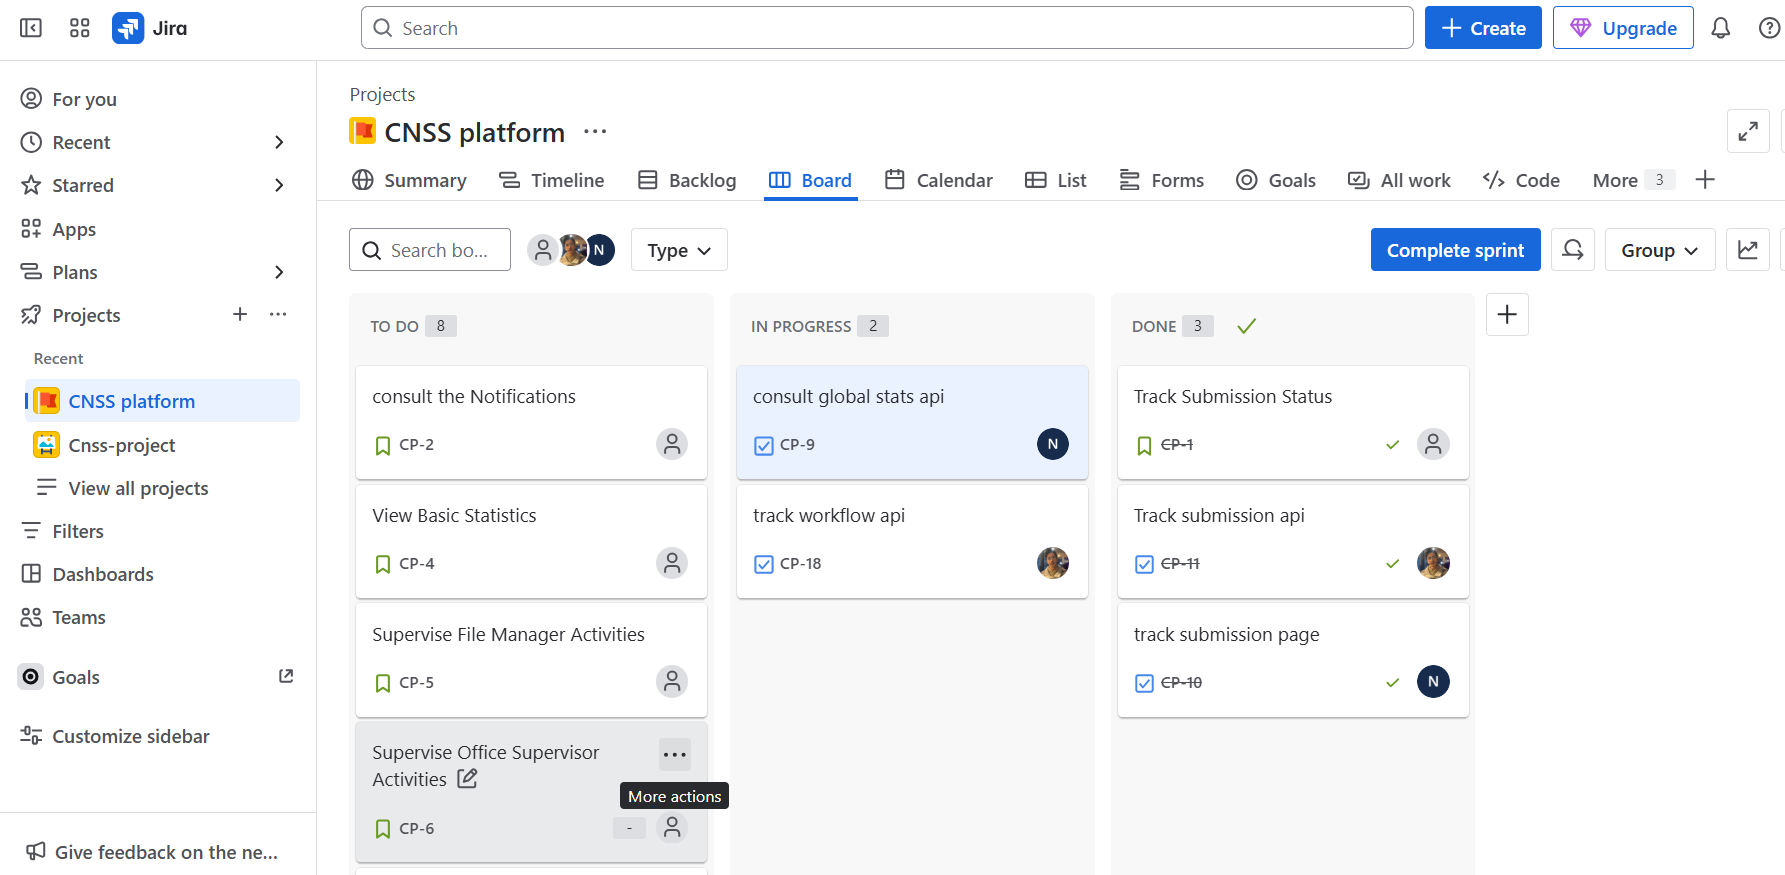
\includegraphics[width=0.9\textwidth]{figures/sprint2 jira.png} 
    \caption{Task distribution for the second sprint using Jira.}
\end{figure}\
\begin{figure}[h]
    \centering
    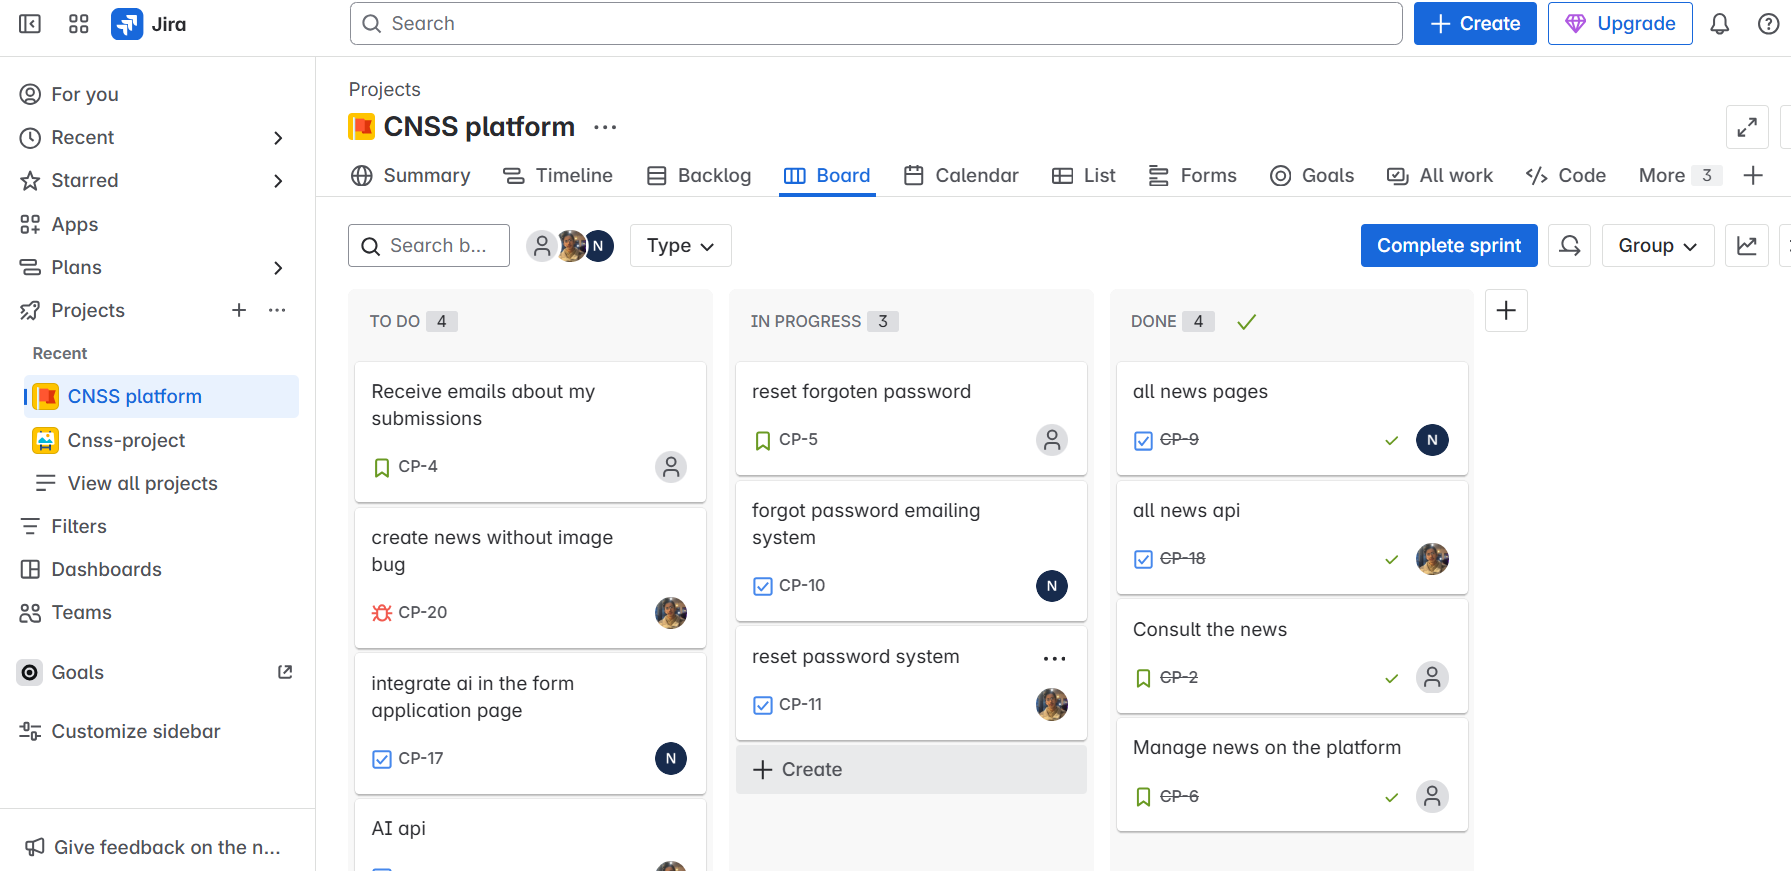
\includegraphics[width=0.9\textwidth]{figures/sprint3 jira.png} 
    \caption{Task distribution for the third sprint using Jira.}
\end{figure}\
\clearpage

\section{Gantt Chart}
A Gantt chart is a project management tool that helps you plan, coordinate, and monitor tasks and their progress within a timeline.
The typical Gantt chart format lists tasks vertically down on the left, while a timeline runs horizontally across the top of the chart. Horizontal bars, or Gantt bars, represent each task's progress, duration, and start and end dates. A Gantt chart also shows milestones, assignees, and dependencies between tasks.\cite{samplewebs31}
\begin{table}[h!]
\centering
\renewcommand{\arraystretch}{1.4}
\rowcolors{2}{rowgray}{white}
\begin{tabular}{|>{\centering\arraybackslash}m{0.6cm}|
                >{\arraybackslash}m{5.5cm}|
                >{\centering\arraybackslash}m{1.5cm}|
                >{\centering\arraybackslash}m{2cm}|
                >{\centering\arraybackslash}m{2cm}|
                >{\centering\arraybackslash}m{1.5cm}|}
\hline
\rowcolor{headerblue}
\textcolor{white}{\textbf{ID}} &
\textcolor{white}{\textbf{Task Name}} &
\textcolor{white}{\textbf{Duration}} &
\textcolor{white}{\textbf{Start}} &
\textcolor{white}{\textbf{End}} &
\textcolor{white}{\textbf{\% Completed}} \\
\hline
1 & Self-training & \textbf{17 days} & 15/01/2025 & 31/01/2025 & 16.19\% \\
2 & Study of the existing system and planning & \textbf{7 days} & 01/02/2025 & 07/02/2025 & 22.83\% \\
3 & Sprint 1: User and candidate management & \textbf{21 days} & 07/02/2025 & 28/02/2025 & 42.83\% \\
4 & Sprint 2: Requests and interview management & \textbf{21 days} & 01/03/2025 & 21/03/2025 & 62.83\% \\
5 & Sprint 3: Validation, notifications, submissions & \textbf{21 days} & 22/03/2025 & 12/04/2025 & 82.83\% \\
6 & Sequence between sprints & \textbf{18 days} & 13/04/2025 & 30/04/2025 & 100\% \\
\hline
\end{tabular}
\caption{Task Allocation Table — Project Schedule (2025)}
\end{table}
\begin{figure}[h]
    \centering
    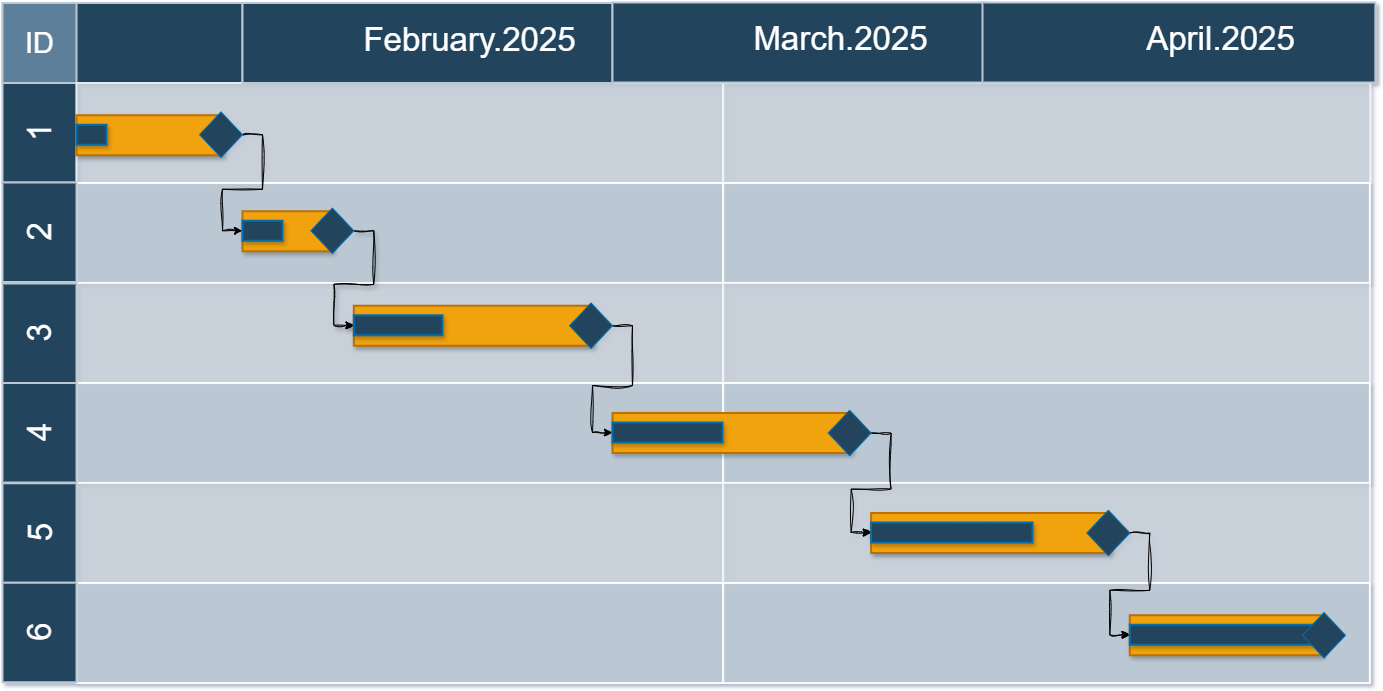
\includegraphics[width=0.9\textwidth]{figures/diagram de gantt.png} 
    \caption{Tasks Diagram.}
\end{figure}\
\clearpage
\begin{center}
    \doublespacing 
    \centering
    \LARGE\textbf{Conclusion} 
    \vspace{1cm} \\
    \raggedright
\end{center}
\addcontentsline{toc}{section}{Conclusion}
Throughout this chapter, we have provided the selection of hardware and software environments used, together with the development tools put in place. 
We have also given screenshots indicating the task distribution across different sprints, as well as the Gantt chart. We conclude our report with this final chapter.